\section{Image Processing of 2D Crystal Images}
\label{sec:single_image_processing}

Electron crystallography of membrane proteins uses cryo-transmission electron microscopy to image frozen-hydrated/sugar embedded 2D crystals. The processing of recorded images exploits the periodic arrangement of the structures in the images to extract the amplitudes and phases of diffraction spots in Fourier space. However, image imperfections require a crystal unbending procedure to be applied to the image before evaluation in Fourier space. Here we describe the image processing of 2D crystal the {\twodx} software system. 

\subsection{Theoretical Background}
\label{sec:2d_background}

The processing of 2D crystal images involves several steps. These steps are the extraction of the lattice, the identification and correction of the crystalline deformation as well as image distortions introduced by the imaging system. This workflow is listed below and simplified in the block diagram in \autoref{fig:2dx_process}.

\begin{figure}[H]
	\centering
	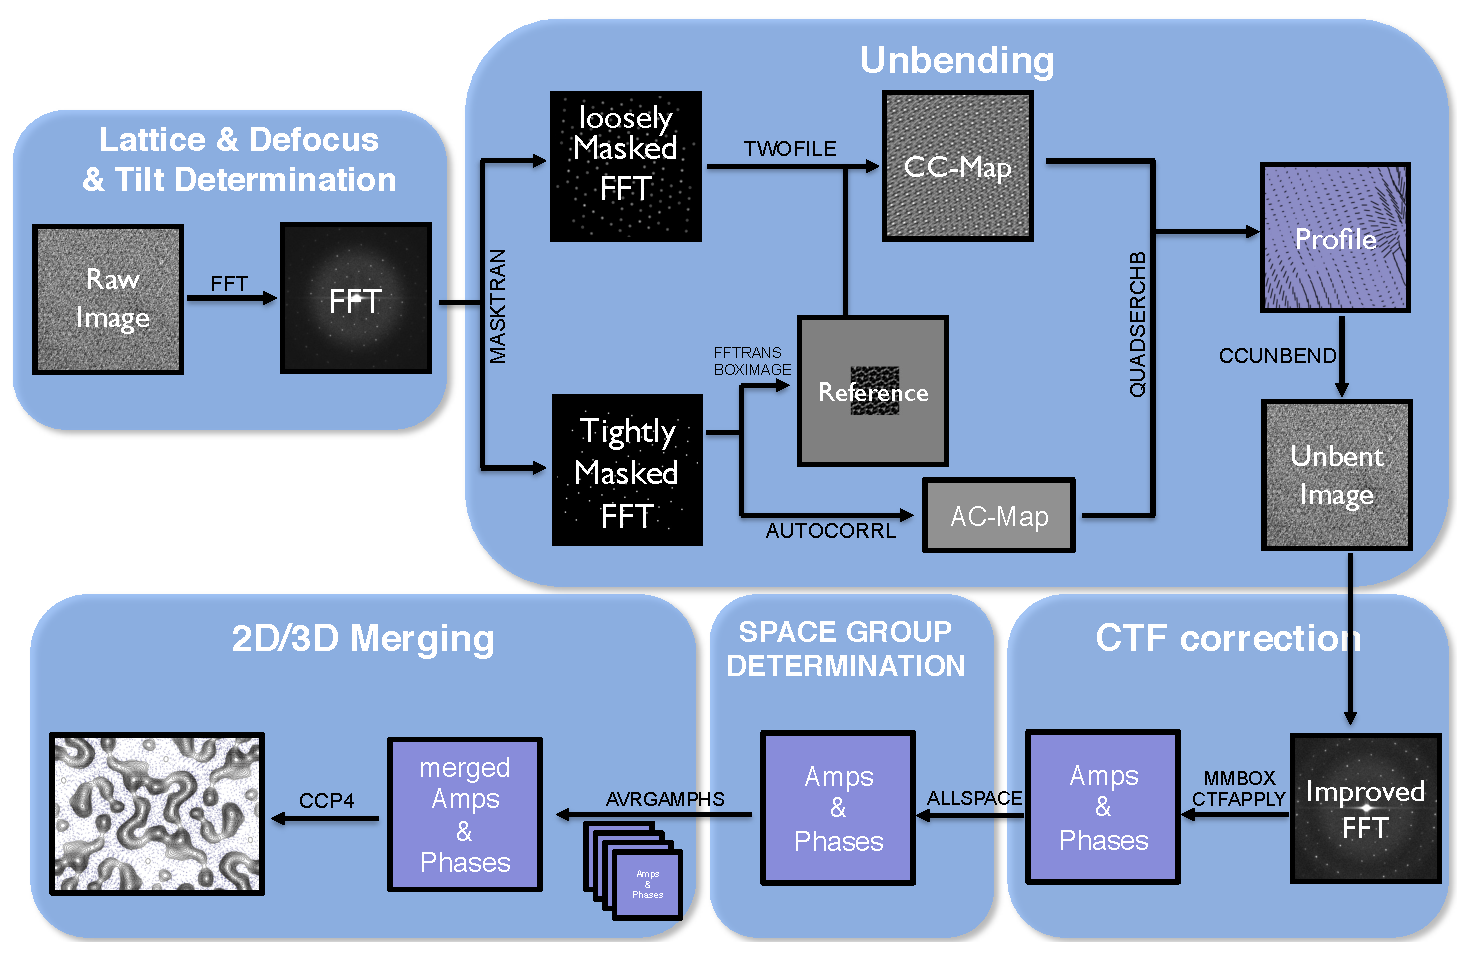
\includegraphics[width=.85\textwidth]{2dx_process.pdf}
	\caption{Single Image Processing Overview}
	\label{fig:2dx_process}
\end{figure}


\begin{enumerate}
	\item Defining basic processing parameters
	\item Calculating the Fourier transform of the image
	\item Measuring the defocus in different locations in the image
	\item Calculating potential specimen tilt from the defocus gradient
	\item Determining the 2D crystal lattice
	\item Calculating potential specimen tilt from distortions of the 2D crystal lattice
	\item Determining a spotlist of significant Fourier reflections
	\item Determine lattice distortion vectors and perform a first image unbending (Unbend I)
	\item Iteratively refine the lattice distortion vectors, do refined unbending (Unbend II)
	\item Extract amplitude and phase values for each Fourier reflection from the unbent image
	\item Correct the list of amplitudes and phases for the microscopes CTF
	\item Determine space group
	\item Calculate a final projection map from this image
\end{enumerate}

These steps will now be discussed in detail, using the 2dx software package as an example. 

\subsection{Getting started}


Starting in {\twodx}\texttt{\_merge} double-click the image that you want to process listed in the Project panel of the graphical user interface. This will open {\twodx}\texttt{\_image} for the selected image. The graphical user interface of {\twodx}\texttt{\_image} consists of different panels displaying data, processing parameters and image-processing routines, as shown in \autoref{fig:2d_overview}. 
	
	\begin{figure}[H]
		\centering
		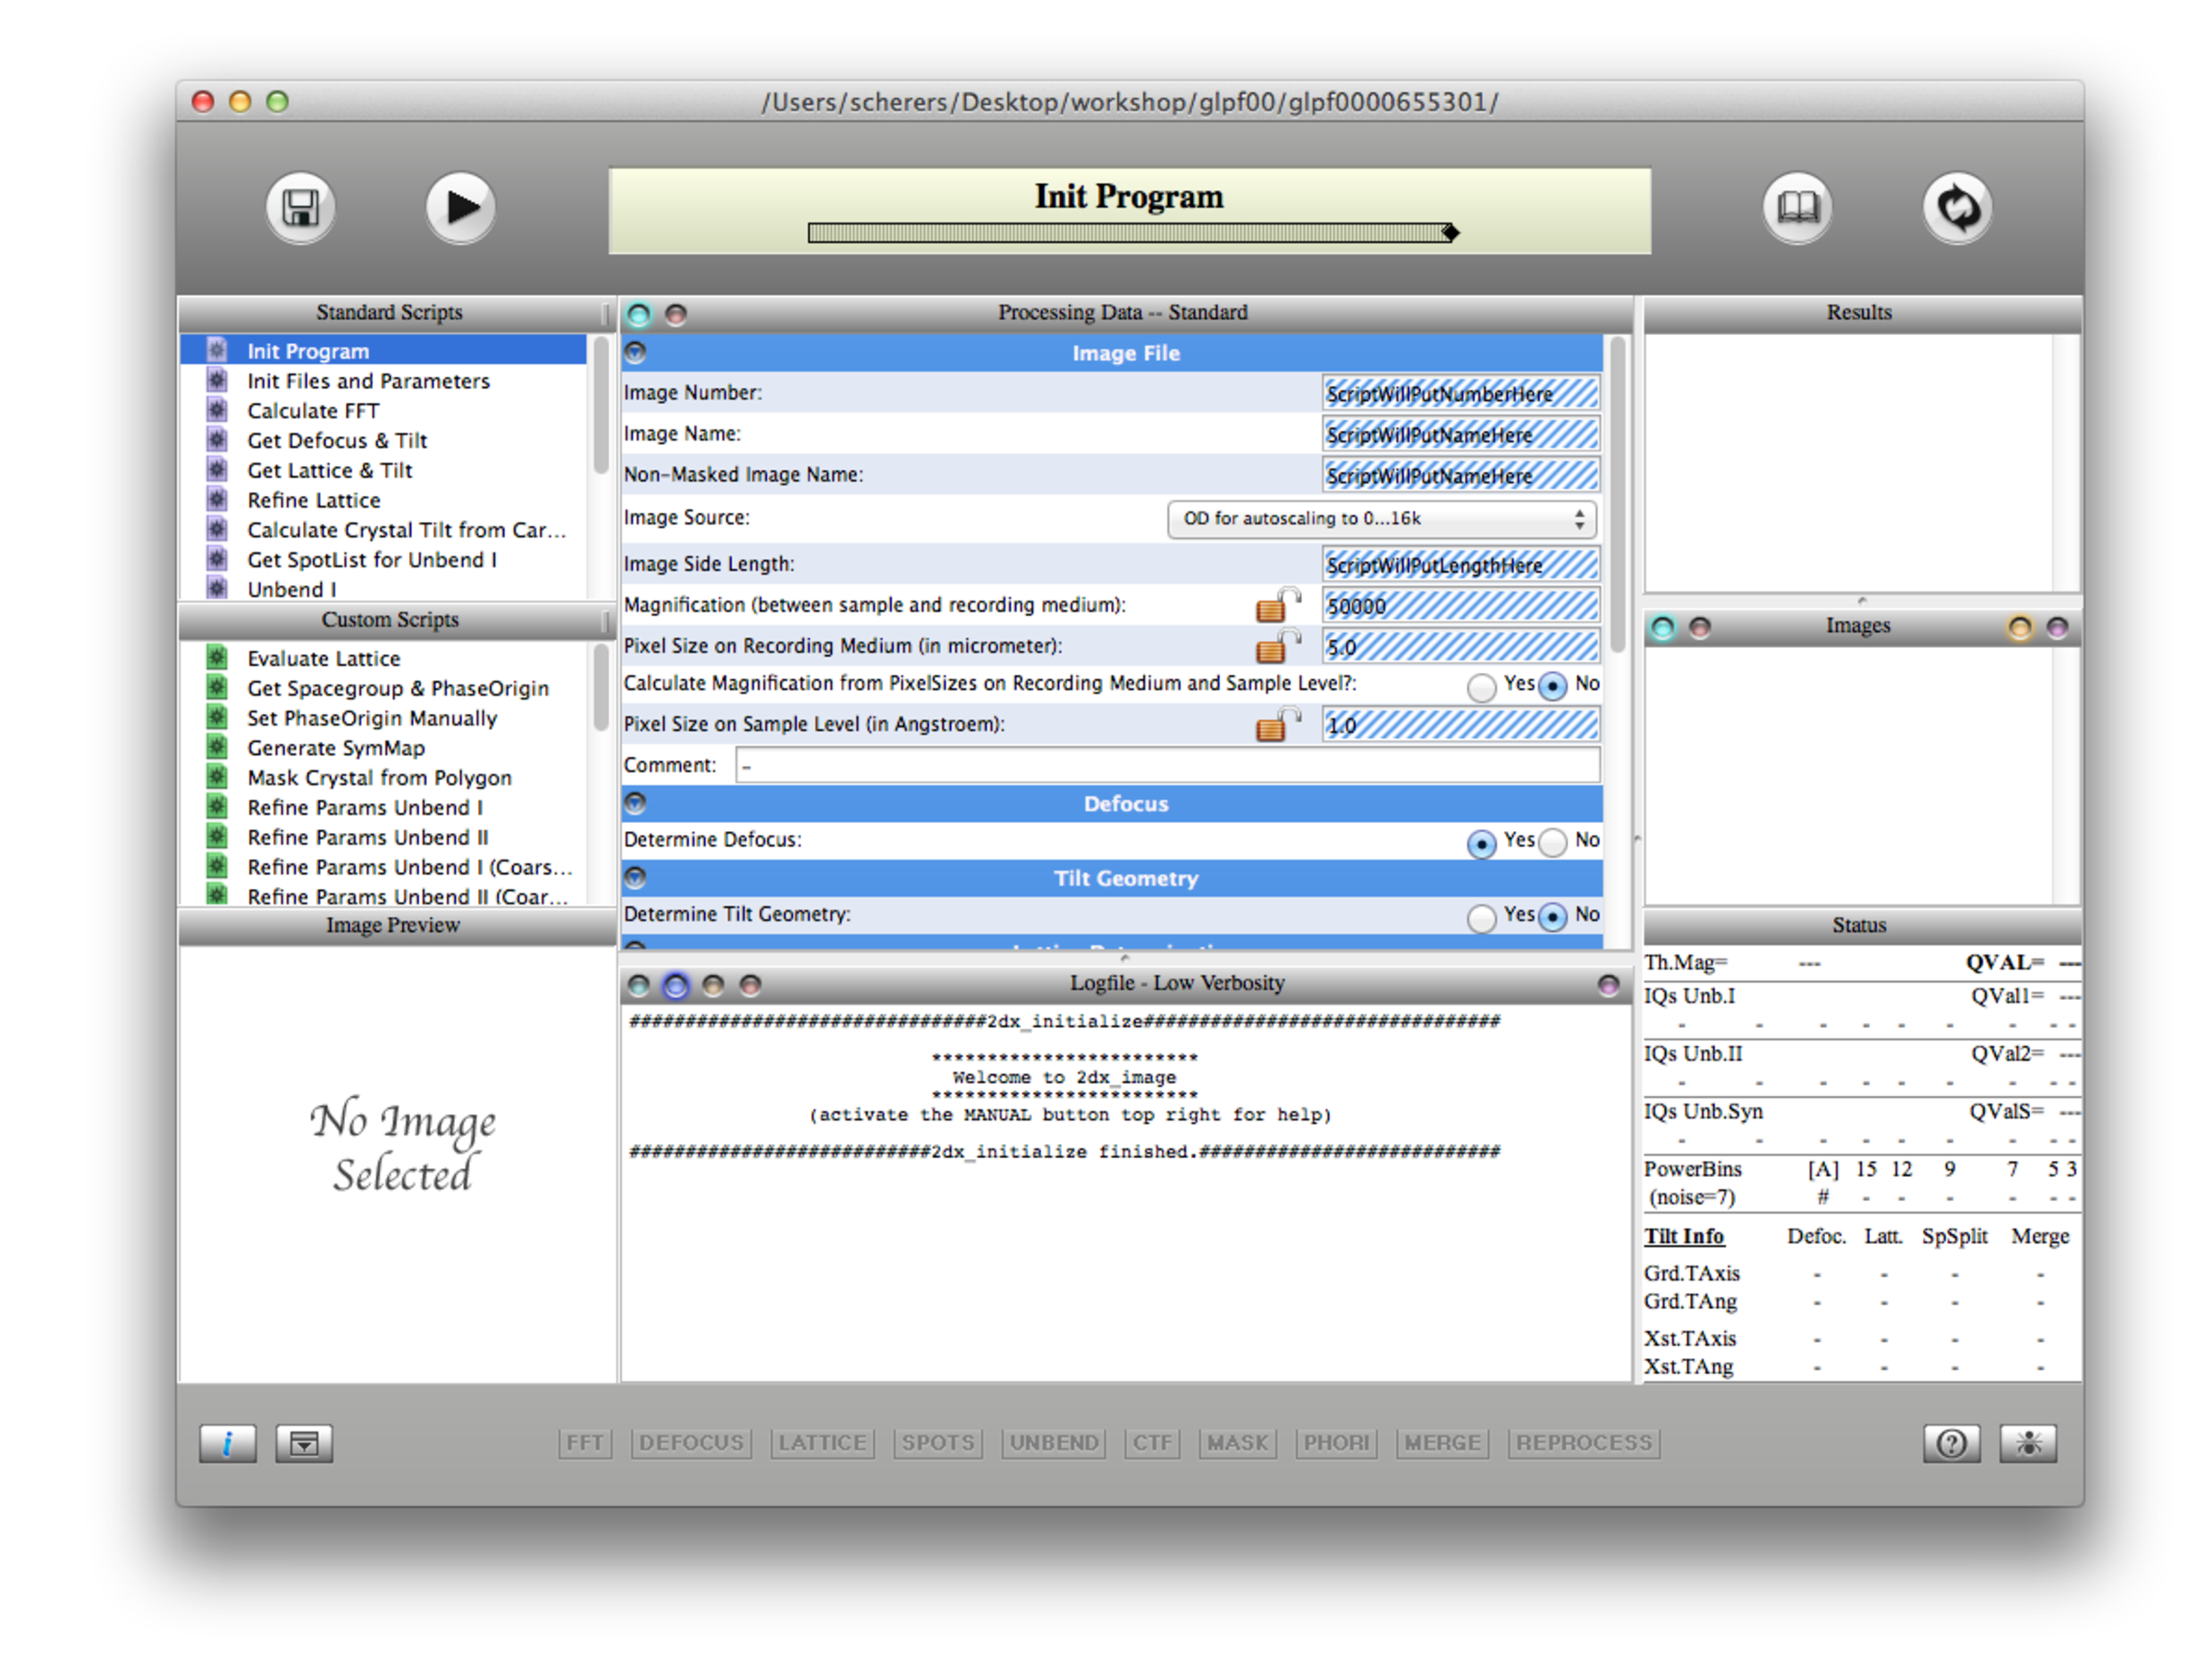
\includegraphics[width=.99\textwidth]{2d_overview.pdf}
		\caption{Individual image processing}
		\label{fig:2d_overview}
	\end{figure}

When {\twodx}\texttt{\_image} is launched it automatically runs the \textit{Init Program} script as displayed by the progress bar in the control panel. The script checks the presence of all required external dependencies and the consistency of the image directory. Next you have to launch the \textit{Init Files and Parameters} script, which prepares the input files for the later processing steps. The image parameters that certainly have to be altered are the \textit{Magnification}, the \textit{Pixel Size on Recording Medium}, \textit{CS} and \textit{kV} value of the used microscope. To save this parameters as default for new imported images click in the menu bar --> File --> \textit{Save as Project Default}. 
If you are unsure what a parameter in the Parameter panel means, you can right click on the according parameter and a description will be displayed, where you also find the link to the online documentation as shown in \autoref{fig:2d_help}. 

\begin{figure}[H]
		\centering
		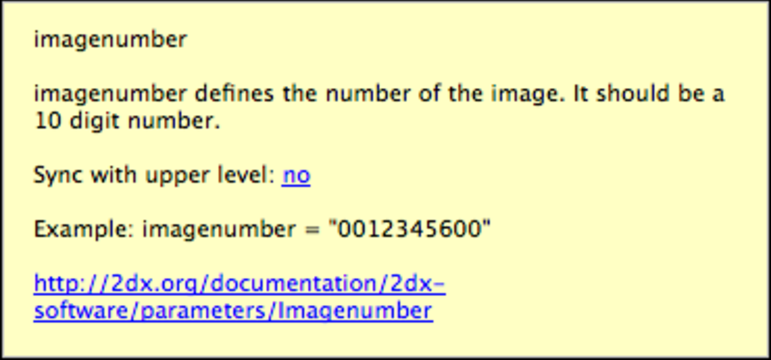
\includegraphics[width=.65\textwidth]{2d_help.pdf}
		\caption{Parameter help window}
		\label{fig:2d_help}
	\end{figure}

On the left of the graphical user interface is the Standard Scripts panel. For every script there is a manual entry that can be displayed when selecting the manual button in the control panel (\autoref{fig:2d_man})
	
	\begin{figure}[H]
		\centering
		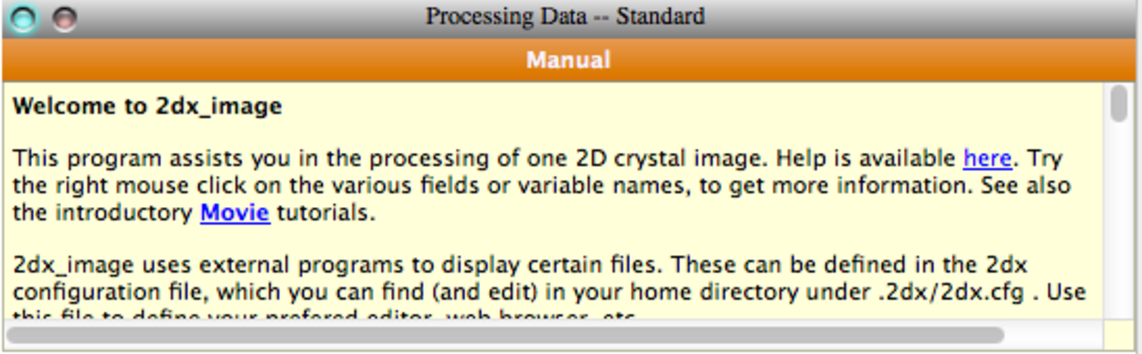
\includegraphics[width=.85\textwidth]{2d_man.pdf}
		\caption{Manual View in {\twodx}}
		\label{fig:2d_man}
	\end{figure}



\subsection{Automated processing}

The image processing workflow of a 2D crystal is in the order of the scripts in the Standard Scripts panel (\autoref{fig:2d_std}). To evaluate the periodicity of the structure the image is transformed into Fourier space, where the lattice is then determined determined in reciprocal space. This lattice is then transformed into real space, and is used to identify the aberrations from the ideal lattice by cross correlating with an idealized reference map. The Contrast Transfer Function (CTF) is then used to correct distortions originated from the imaging.
	
	\begin{figure}[H]
		\centering
		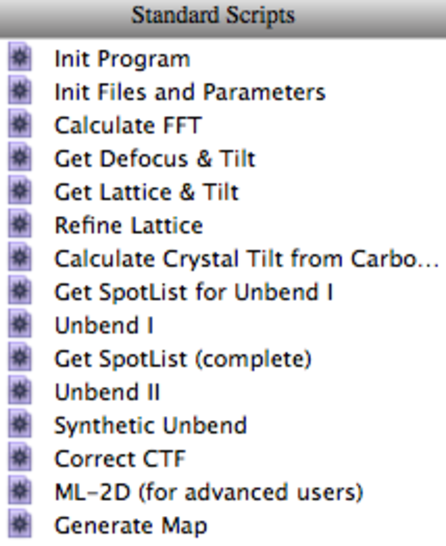
\includegraphics[width=.4\textwidth]{2d_std.pdf}
		\caption{Standard scripts in {\twodx}\texttt{\_image}}
		\label{fig:2d_std}
	\end{figure}
	
Since {\twodx}\texttt{\_image} is able to process the image in automated manner, select all the scripts in the Standard Scripts panel and press the \textit{Play} button in the control panel.
The scripts are executed consecutively. The progress bar depicts, which script is running momentarily and the Log panel displays the text output of the running script. You can change the verbosity level of the output in the Log panel with the buttons in the left corner of the panel.
When {\twodx}\texttt{\_image} has ran all scripts click on the last script of the workflow \textit{Generate Map} to see its outcome. The result of the automatic unbending and CTF correction can be examined by double-clicking the \textit{Non-symmetrized Map} in the Images panel. This will display $2 \times 2$ unit cells.


\subsection{Manual processing}
Since the automatic processing is not perfect you may want to improve your result manually. You can do this in {\twodx}\texttt{\_image} at any time and will still profit from the prior executed steps.
In this section we will walk you through each step. 

\subsubsection{Determine defocus}
\label{sec:defocus}
\index{Determine Defocus}

The first step is to determine the defocus and astigmatism for the later CTF correction. To do so run the  \textit{Calculate FFT}  and the \textit{Get Defocus}\index{Get Defocus} script and double click on \textit{FFT of Downsampled Image} in the Images panel. This will open up a down sampled Fourier transformation of the original image in the full screen viewer. You can zoom in with the period key and out with coma key. Press "C" in the full screen browser or select \textit{View CTF} in the \textit{Navigator} menu to see the Thon rings. You can adjust the defocus and astigmatism in the dialog window as shown below in \autoref{fig:2d_defocus}.
	
	\begin{figure}[H]
		\centering
		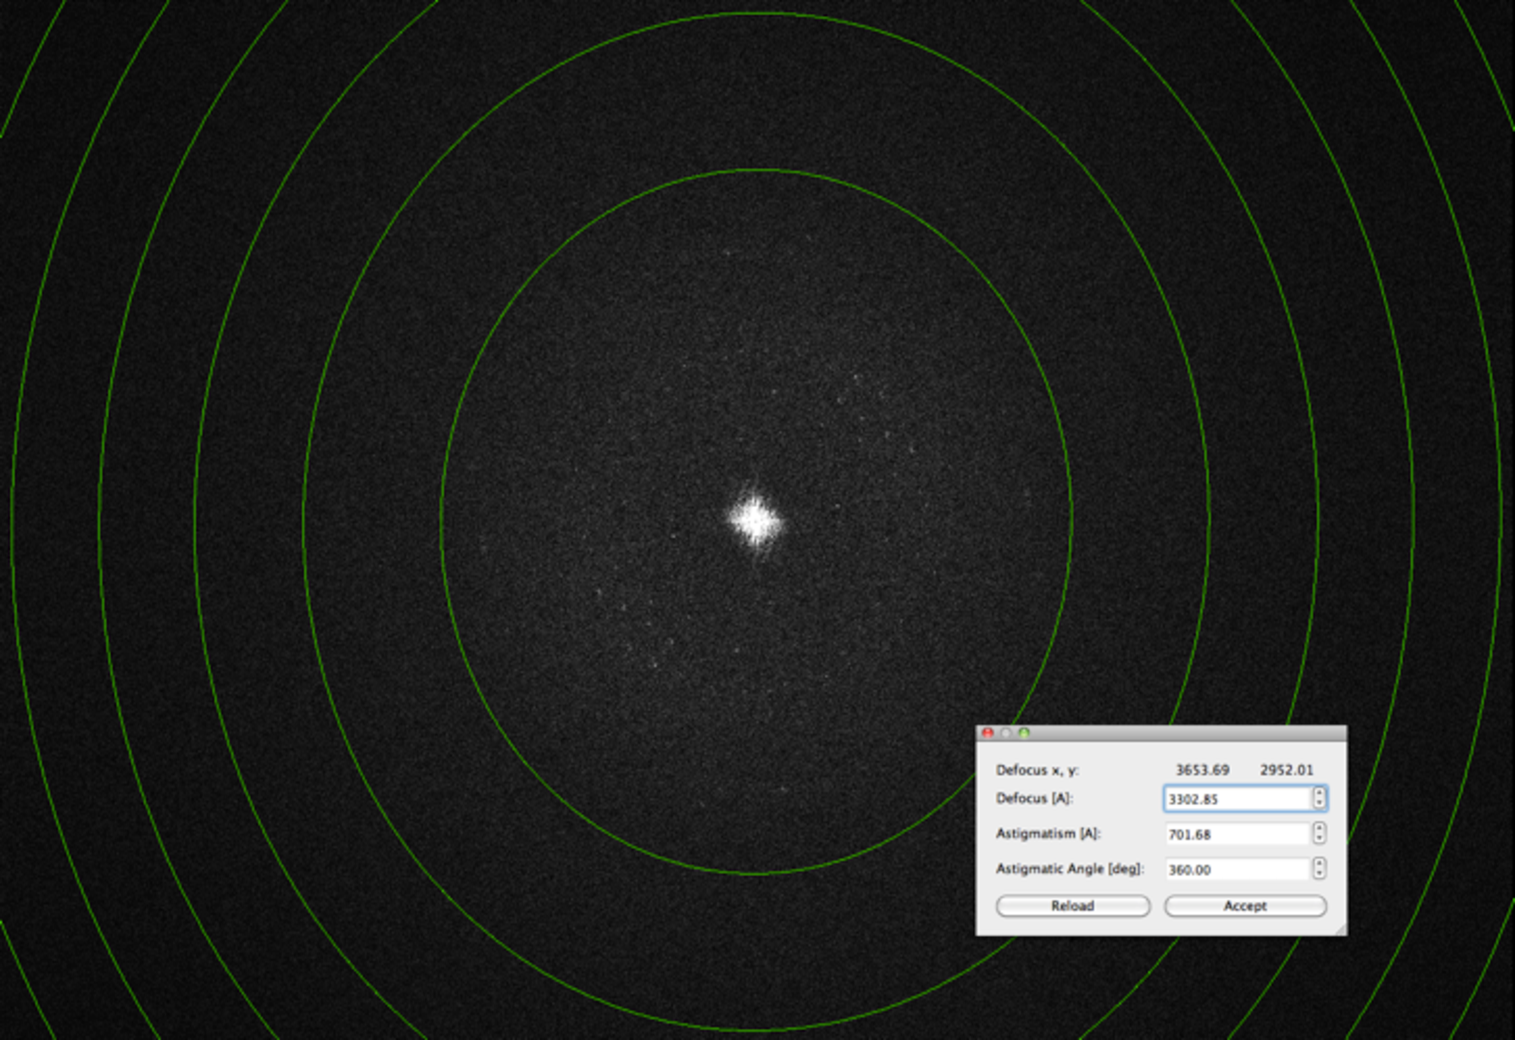
\includegraphics[width=.99\textwidth]{2d_defocus.pdf}
		\caption{Determine the best defocus of an image}
		\label{fig:2d_defocus}
	\end{figure}

	If you have trouble seeing the Thon rings you may want to change the Brightness and the contrast in the full screen viewer. You can do so by selecting \textit{Adjust Contrast/Brightness} dialog from the \textit{Navigator} menu. Press \textit{Accept} if you are happy with the parameters, or use the shortcuts "B" and "N".
	
	If you still have problems seeing the Thon rings you can create a peridogram. To do enter the \textit{Advanced} view in the Parameter panel of the \textit{Calculate FFT} script by clicking the right button in the upper left corner of the panel. This will give you the full parameters list. Select \textit{Yes} for \textit{Generate periodogram?} and run the script again. The periodogram will show up in the Images panel and in this image you might see the Thon rings more clearly and can select them more easily. The selection is made in the same matter as before. 
	
	The defocus and astigmatism values will be used later in the \textit{Correct CTF} script.
	
\subsubsection{Determine lattice}	
	
The next step is to determine the crystal lattice. You can run the \textit{Get Lattice \& Tilt} script in order to find automatically your lattice. Open \textit{FFT of Downsampled Image} in the full screen browser. You can display the lattice by pressing the "L" key.
By pressing the D key or selecting \textit{Display Coordinate Info} from the \textit{Navigator} menu, you will get a dialog window that displays the amplitude, phase, the Miller index etc. of the pixel that the mouse pointer hovers over. To define the lattice de novo or to refine the lattice you have to enter the \textit{Lattice Refinement Mode} through the \textit{Lattice Refinement} in the \textit{Navigator} menu as shown in \autoref{fig:2d_lat}.
	
	\begin{figure}[H]
		\centering
		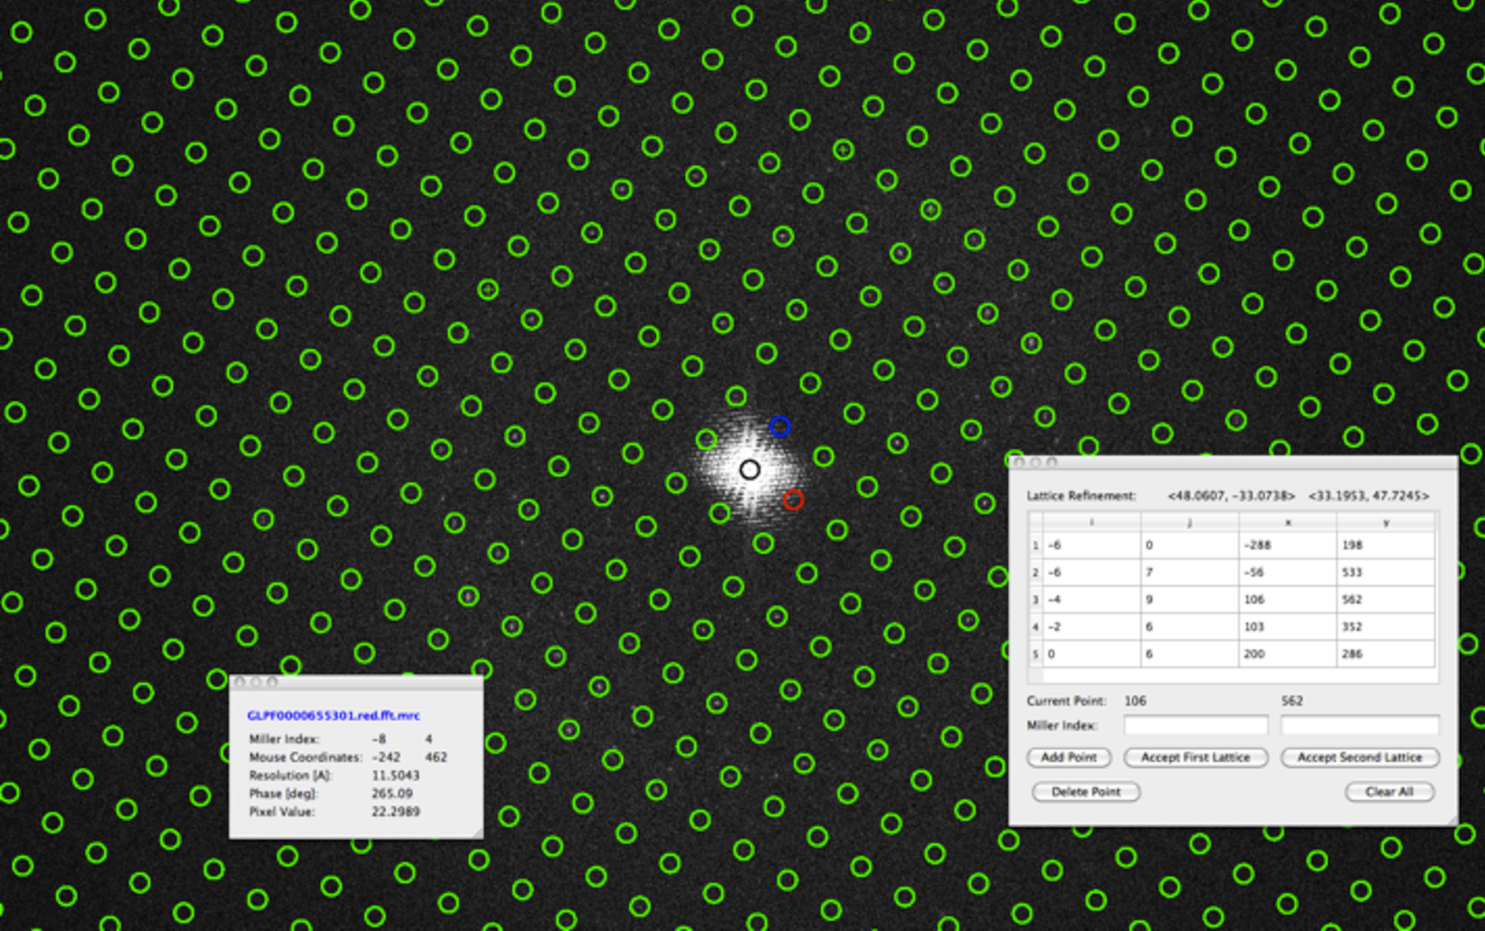
\includegraphics[width=.99\textwidth]{2d_lat.pdf}
		\caption{Lattice of an image}
		\label{fig:2d_lat}
	\end{figure}
	
	Now you are able to add spots to your lattice. These would ideally be spots with a high resolution. With a double click the spot with the maximum intensity value in the surrounding area of your mouse pointer is selected. By pressing the Enter key or the \textit{Add Point} in the \textit{Lattice Refinement} dialog window the spot is added to the table. The Miller index is chosen according to the existing lattice. In case this is wrong you can alter it in the dialog window. You can activate the \textit{Display Parameters} dialog window in the Navigator window. Here you can change the \textit{Maximum Value Search Range} that is used when double clicking. Or you can change the method to use a \textit{Gauss Fit}. To get a closer look at the area you can make a right click. 
	
After having added spots press the \textit{Accept First Lattice} button and you will see how the lattice is shifted to match the picked spots.
	
Ideally you will have only one lattice. But usually there is a second weaker lattice showing in Fourier space. This lattice can be defined and refined in the same manner as with the first lattice. You can view this lattice by pressing the S key. The second lattice could later be used to filter out spots that overlap in the process of unbending.

You can calculate the unit cell dimensions which is defined by this lattice by running  the \textit{Evalute Lattice} script from the Custom Scripts panel.




\subsubsection{Determine tilt geometry}
\label{sec:det_tilt}
\index{Determine tilt geometry}



If you are processing a non-tilted image you should set \textit{Determine Tilt Geometry} to \textit{No} in the \textit{Tilt Geometry Section} of the Processing Data panel.
In case you are processing a tilted image there are two ways to determine the tilt geometry of your image. Firstly, you can determine the tilt geometry from the defocus gradient  of your Fourier transform (see \autoref{fig:tilt_1}). This will be executed together with the \textit{Get Defocus \& Tilt} script. This way you determine the tilt geometry of the carbon film support, which is described by the variables TLTAXIS (tilt axis of the microscope) and TLTANG (angle between tilt axis and the grid). These two variables are valid for the sample support, and have nothing to do with the crystal. In fact, they could also be determined in absence of any crystal. Please note, that for smaller tilt angles, the defocus gradient is the safer method.

\begin{figure}[H]
		\centering
		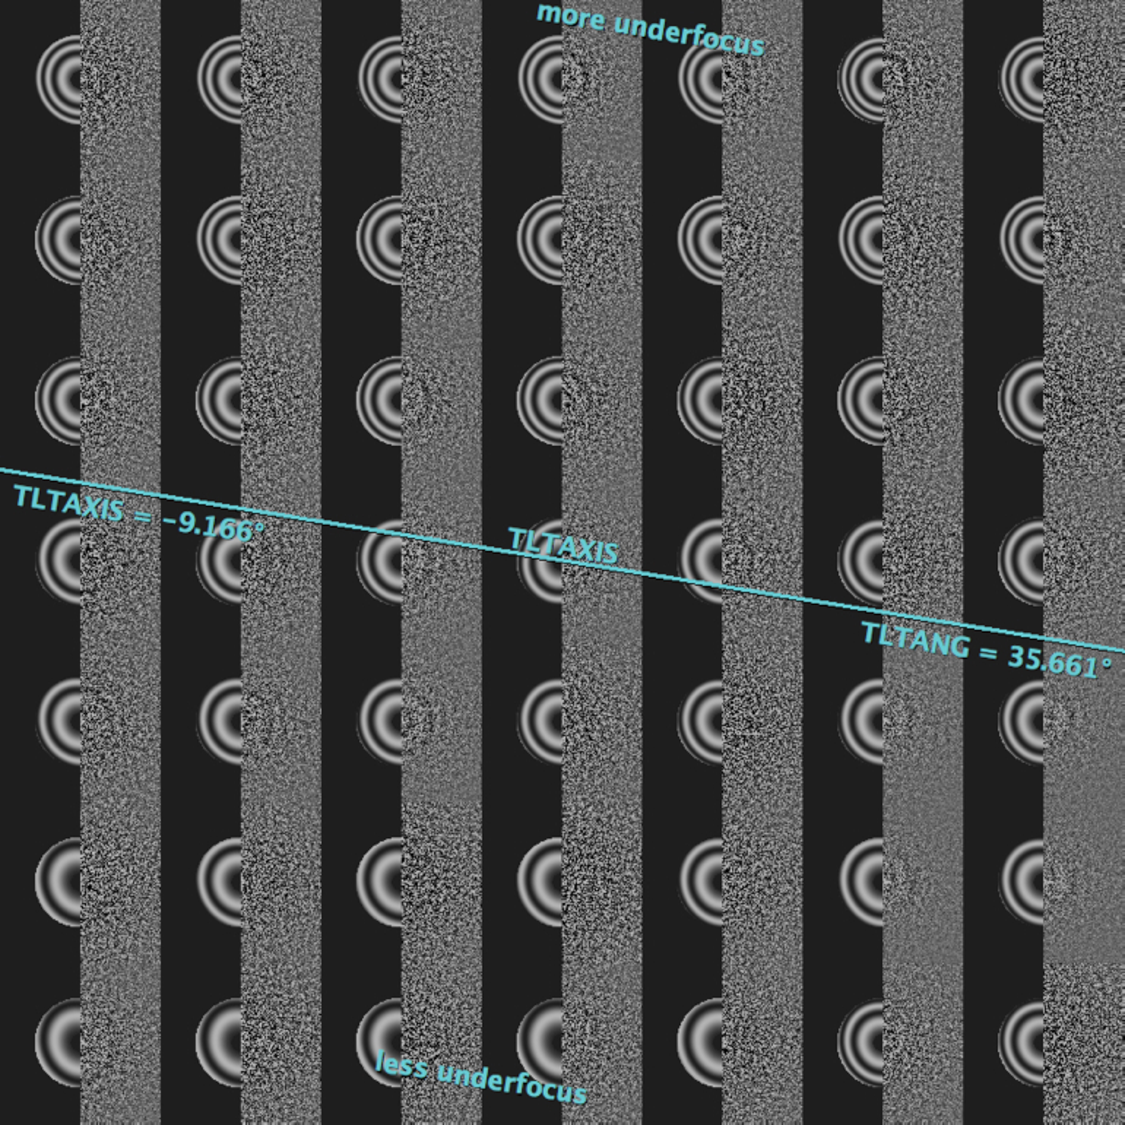
\includegraphics[width=.99\textwidth]{tilt_1.pdf}
		\caption{Determining tilt geometry from the defocus gradient.}
		\label{fig:tilt_1}
	\end{figure}
	

Secondly, you can determine tilt geometry based on the lattice distortion. For this purpose you have first to define the lattice, for example after running the \textit{Get Lattice \& Tilt} script. 
In addition to the TLTAXIS and the TLTANG it will also calculate TLTAXA, which describes the orientation of the crystal with respect to the tilt axis (see \autoref{fig:tilt_2}).
This lattice-based tilt geometry is only reliable for larger tilt angles, which should be greater than 25 degrees. In that case, the \textit{Get Lattice \& Tilt} script will use the now determined lattice orientation to translate the defocus-based tilt geometry into the sample tilt geometry.

\begin{figure}[H]
		\centering
		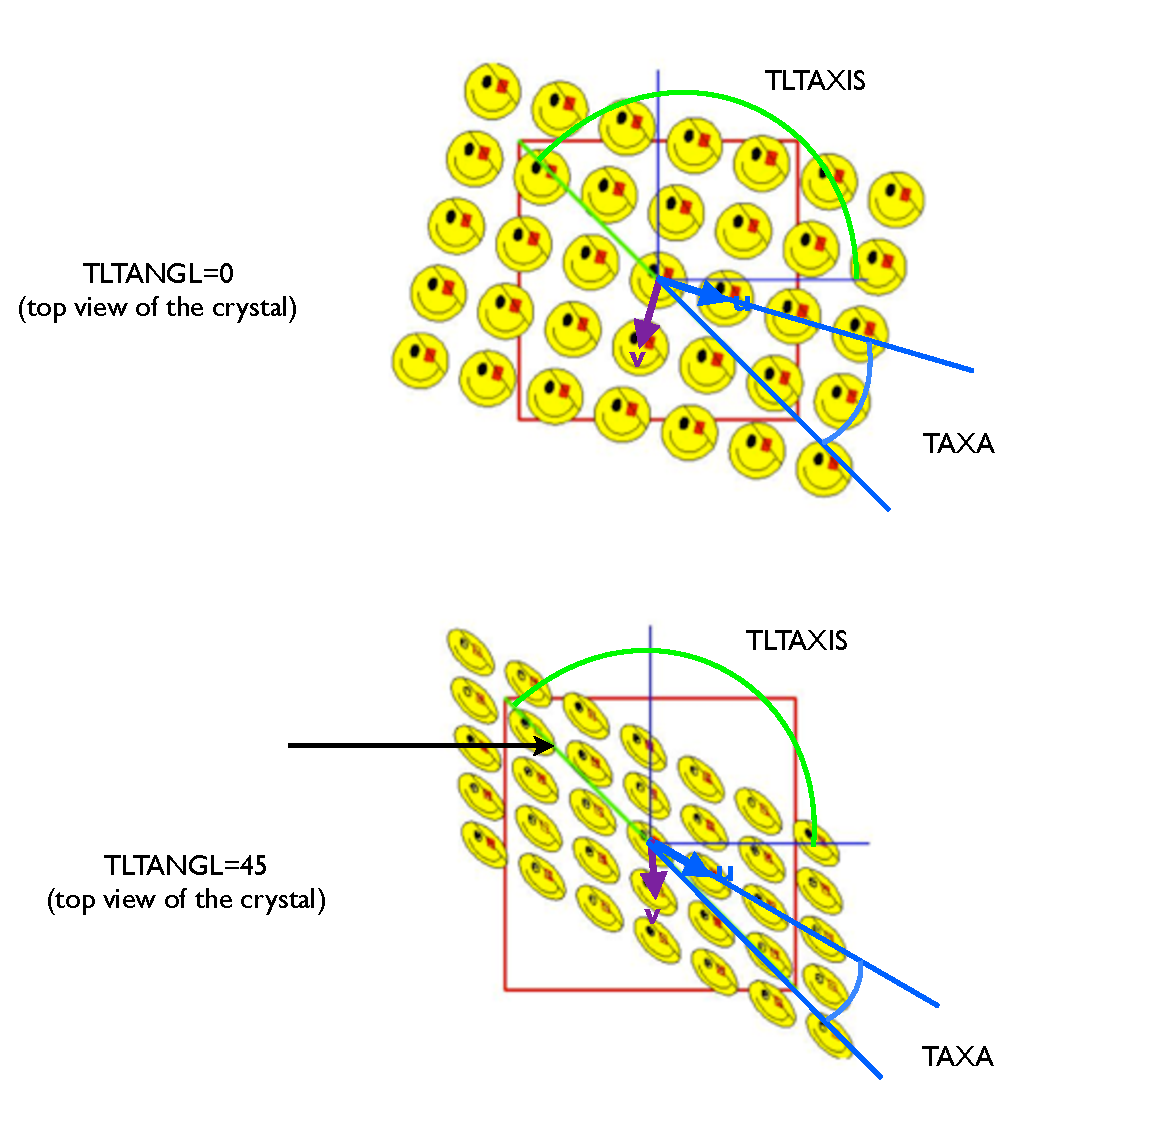
\includegraphics[width=.99\textwidth]{tilt_2.pdf}
		\caption{Determining tilt geometry from the lattice distortion.}
		\label{fig:tilt_2}
	\end{figure}
	



\subsubsection{Determine reference area}
\label{sec:reference}
\index{Determine reference area}	

For the upcoming unbend processes you need to define a reference, which should be the best crystalline area of your image. If the image recording and scanning was done carefully the centre will be close to the actual centre of the digitized array. Nevertheless, checking the live-FFT on your image is often beneficial, especially for specimens that are not perfectly ordered. Should this not be the case you can select your reference area manually. 
Open the \textit{Non-Masked Image} in the Image panel. This will show the source image in the full screen viewer. You can zoom in on the image with the comma key, and zoom out with the period key or via the menu. Zoom out to see the full picture. Right-click on the image under \textit{Selection based FFT} select \textit{FFT of Selection} as shown in \autoref{fig:2d_fftmenu}. 
	
	
		\begin{figure}[H]
		\centering
		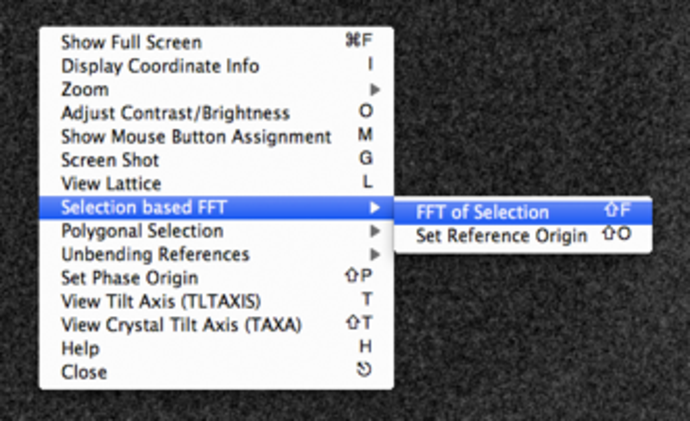
\includegraphics[width=.65\textwidth]{2d_fftmenu.pdf}
		\caption{FFT Menu}
		\label{fig:2d_fftmenu}
	\end{figure}
	
	Now you can select a rectangular area on the image by dragging the left-mouse button and the Fourier transformation of the selection is then displayed. You can also displace the selection with the right mouse button. The corresponding screenshot is shown in \autoref{fig:2d_fft}.

	\begin{figure}[H]
		\centering
		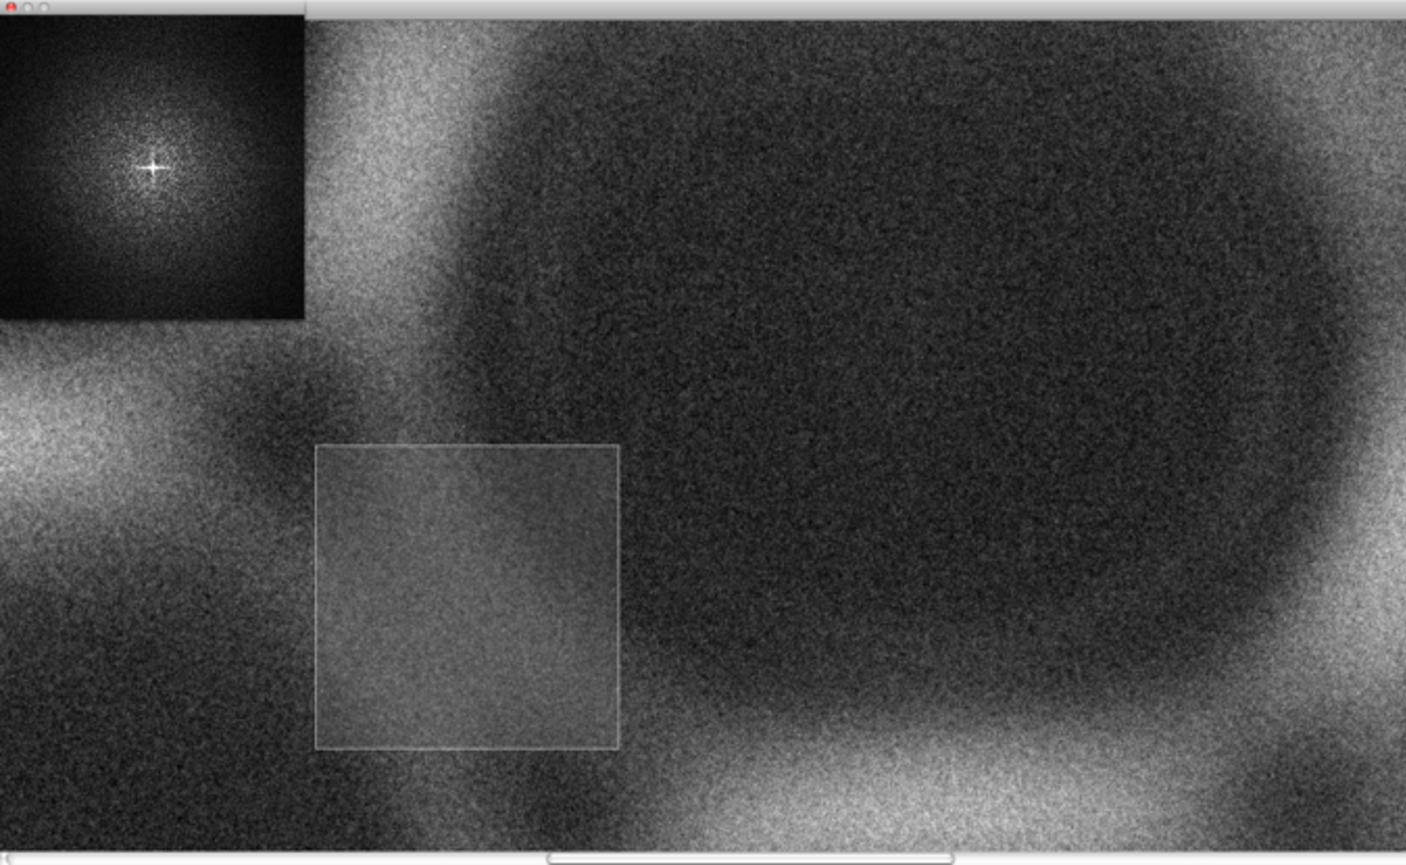
\includegraphics[width=.99\textwidth]{2d_fft.pdf}
		\caption{FFT live view}
		\label{fig:2d_fft}
	\end{figure}
	
Select the best area, which should show the best/most spots on the live FFT. Press the "I" key to note the coordinate. Leave the full screen viewer (press Escape) and return to the main window. Insert the coordinates of your chosen reference area in the \textit{Get Spotlist for Unbend I} script. 



\subsubsection{Unbend}
\label{sec:Unbend}

This chapter describes how you can correct for translational crystal distortion in {\twodx}\texttt{\_image}. Therefor you compare (= cross-correlating) a tightly masked and thus "perfect" transform (= reference) with a loosely masked transform that still contains all the information about irregularities in the lattice. However, to get the best results one first needs to determine the xy-coordinates that will serve to centre the reference area (see  \autoref{sec:reference}). The cross-correlation is done most conveniently in reciprocal space (\texttt{twofile}) because in this case it amounts to a multiplication of the loosely masked transform of the image with the complex conjugate of the transform of the reference area. Backtransformation of the cross-correlation map is the first step to translate its information into real space disorder parameters. Consecutively, all unit cells can be searched for the exact position (= offset) of the object and the degree of similarity with the reference area (\texttt{quadserchb}). In practical terms this is achieved by first correlating the object (or part of it) with itself. This so called autocorrelation map is calculated from a small part of the reference area and its centre appears as a more or less symmetrical peak whose shape depends on the actual distribution of Fourier terms in the image (\texttt{autocorrl}). Finding the best fit of this central peak and the cross-correlation peaks for the individual unit cells provides the length and orientation of the distortion vectors and goodness (=height) of correlation. It should be mentioned that \texttt{quadserchb} only determines the translational offset for the cross-correlation peak but does not take into account any rotational disorder. Once the distortion vectors are known, the original image can be corrected by re-interpolating its optical densities to bring the unit cells onto a "perfect" lattice (\texttt{ccunbend}). The resulting unbent image is Fourier transformed to give an FFT with sharper diffraction peaks. The unbent FFT is evaluated (\texttt{mmbox}), yielding a list of amplitudes and phases for each lattice spot, together with an IQ value for each spot, which express the signal-to-noise ratio. The weighted sum of all IQ spots is depicted in the QVal, which can be used to judge the quality of the results of image processing.

\begin{figure}[H]
		\centering
		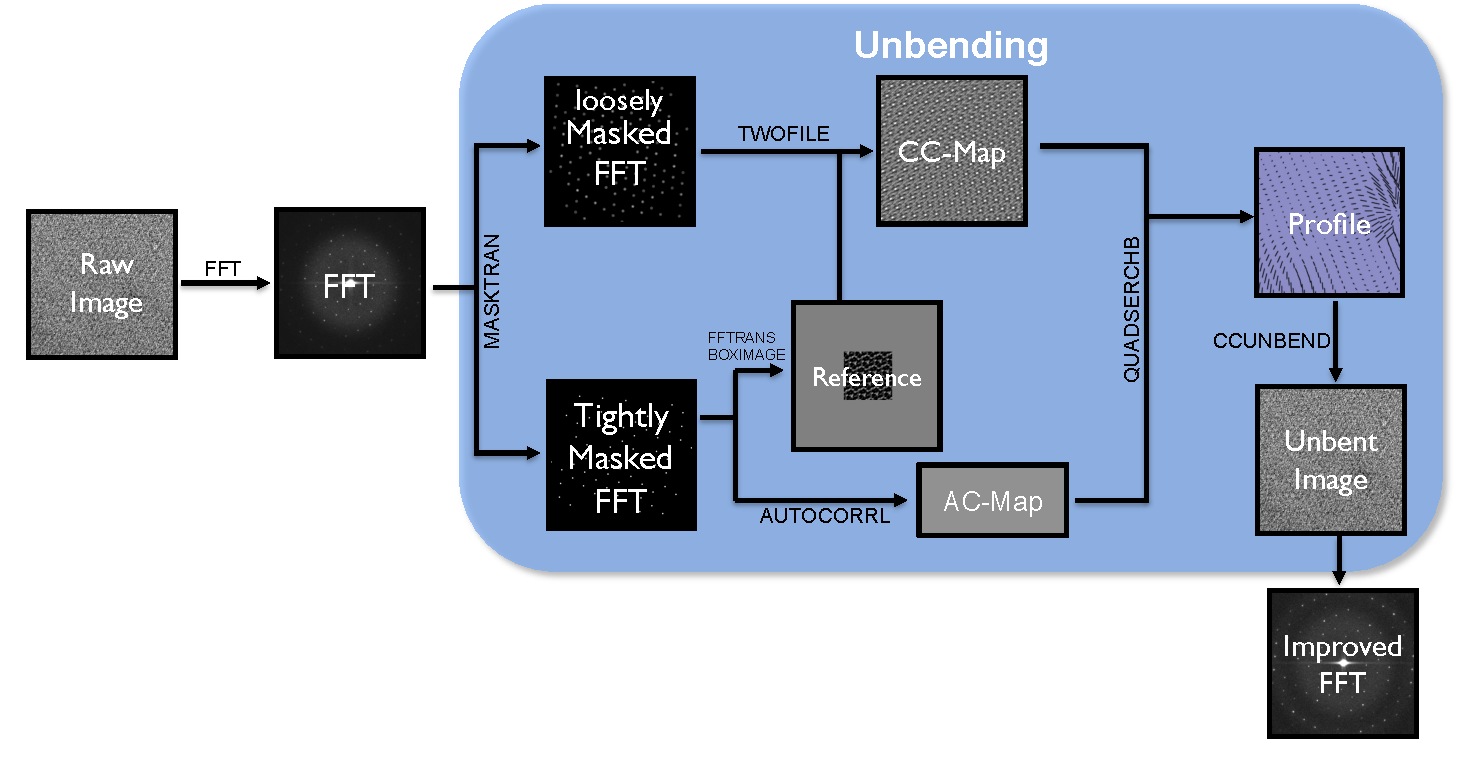
\includegraphics[width=.99\textwidth]{unbendprocess_1.pdf}
		\caption{Overview of the unbend process.}
		\label{fig:unbendprocess_1}
	\end{figure}



The unbending is split into two rounds as depicted in the Standard Scripts panel by the \textit{Unbend I} and \textit{Unbend II} scripts. The needed reference for each unbending step is created from a spot list, which holds spots in Fourier space that lie on the lattice (scripts \textit{Get Spotlist for Unbend I} and \textit{Get Spotlist complete}. You can manually refine this spot list in the full screen view of the Fourier transformation. Enter \textit{Spot Selection Mode} via \textit{Spot Selection} in the Navigator Menu. With the P key you can identify the spots automatically selected. You may want to display the lattices when refining the spots (\autoref{fig:2d_spot}). By clicking on a lattice spot you select it and by clicking it again you undo the selection. In this manner select now the spots that have a high signal to noise ratio.
Save the spot list under \textit{Spot List} in the \textit{Navigator} menu.
	
	\begin{figure}[H]
		\centering
		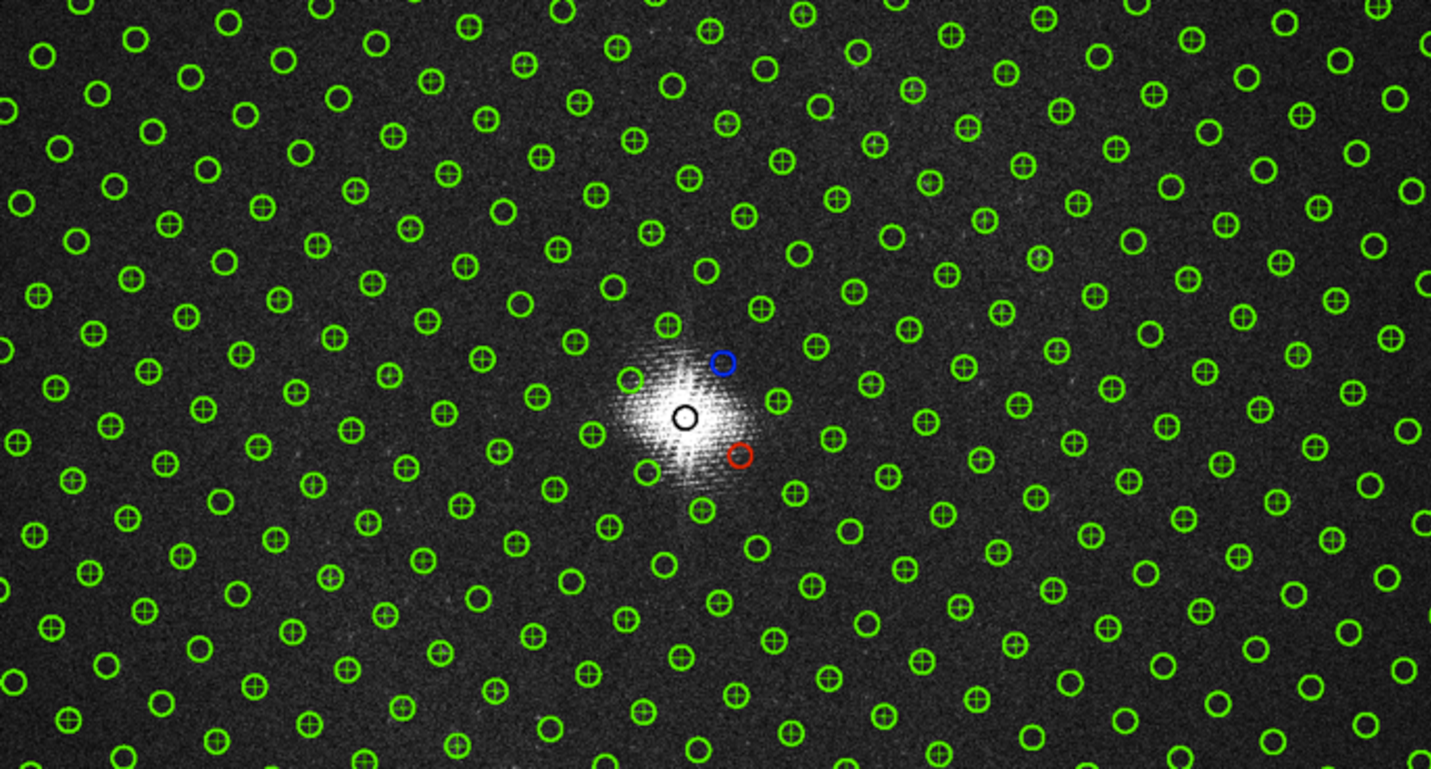
\includegraphics[width=.99\textwidth]{2d_spot.pdf}
		\caption{Spot refinement mode}
		\label{fig:2d_spot}
	\end{figure}


From this outline it becomes clear that the quality of the reference area is the main factor to the success of the "unbending" procedure because any disorder present in the reference will remain uncorrected. Accordingly, improvements in the quality of the reference area by successive passes of processing make the determination of the lattice distortions and consequently, the correction of the image more accurate. In most cases the result will not get any better after 2-3 passes of image filtering and lattice unbending. However, a further improvement can be obtained once a 3D model is available, because in this case a "perfect" reference area can be created de novo by calculating a back projection of the model for the "precise" imaging conditions (\texttt{maketran}, see \autoref{sec:syn_unbending}). Further parameters you can play around with are the radius of the loosely masked Fourier (\textit{mask}) and the diameter of the reference (\textit{box}).

	
\newpage

\subsubsection{Crystal masking}
\index{Masking}
\label{sec:masking}

In real world applications the crystal almost never fills the entire image as shown in \autoref{fig:mlk01}.

\begin{figure}[H]
	\centering
	\includegraphics[width=.85\textwidth]{mlk01.pdf}
	\caption{Non perfect crystal}
	\label{fig:mlk01}
\end{figure}

Therefore it does not make sense to use regions where the crystal is not regular or where we don't have any crystalline structure. {\twodx}\texttt{\_image} offers a tool with which you can manually mask an image. The following walkthrough explains how you can mask the crystal.


\begin{enumerate}
	\item There are multiple ways how you can mask your image. You can mask the crystal automatically by selecting the option \textit{Do automatic masking of 2D crystal} in the Parameter panel of  \textit{Unbend II}. 
Alternatively, you can mask your crystal manually.  Open the original image from the result panel of the initialization script and mask the image there. For many applications this does not work, as the crystal is not visible by eye. Thus we advise to mask in the file \textit{XCF Map for Manual Merging} which can be found in the result panel of \textit{Unbend II}. This file shows you the cross-correlation profile generated during unbending the crystal. The height of the peak corresponds directly to the local quality of the crystal. In regions with no crystalline structures we will not find any peaks. As usual the file is opened in the fullscreen mode by a simple double click. 	
	\item In order to be able to mask the image you have to activate the \textit{Polygon Selection Mode} by right-clicking in the image and selecting "Polygon Selection > Polygon Selection Masking" as shown in \autoref{fig:mask_2}.

	\begin{figure}[H]
		\centering
		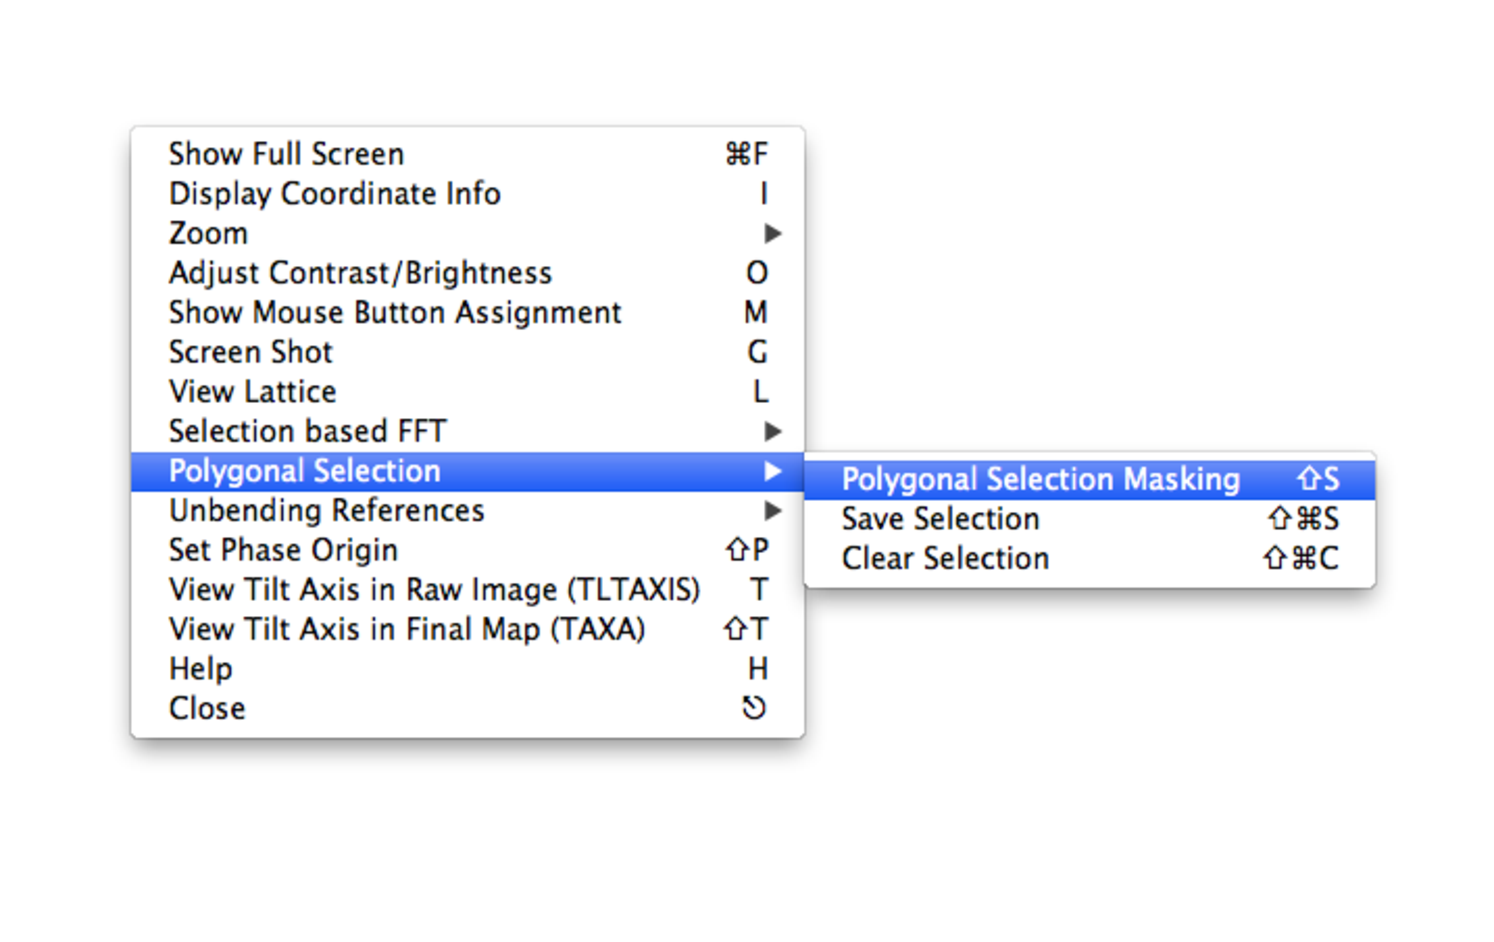
\includegraphics[width=.85\textwidth]{mask_2.pdf}
		\caption{Activate the Polygonal Mode}
		\label{fig:mask_2}
	\end{figure}
	
	\item Now you can mask your crystal by defining the borders with a bunch of left mouse clicks. A double-click will automatically close the selected polygon. Note that you can delete the current selection by selecting "Polygon Selection > Clear Selection" from the menu appearing when right-clicking on the image. Your masked image should be somehow similar to \autoref{fig:mask_3}.
	
	\begin{figure}[H]
		\centering
		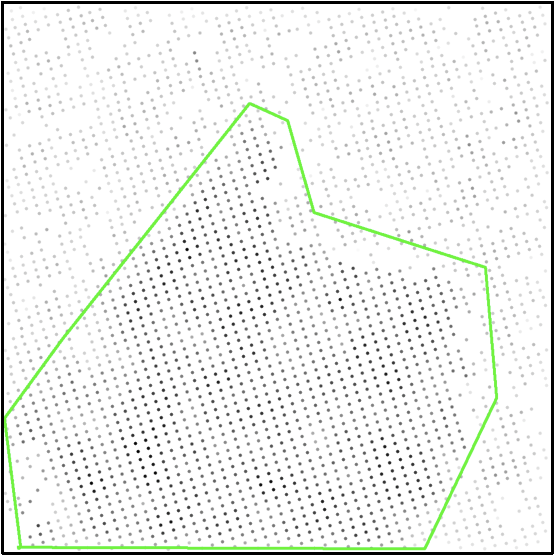
\includegraphics[width=.85\textwidth]{masked.pdf}
		\caption{Masked XCF Map}
		\label{fig:mask_3}
	\end{figure}
	
	\item Once you are happy with your selection you can save the current selection by selecting "Polygon Selection > Save Selection" from the menu appearing after another right-click.

	\item In order to apply your polygon selection you have to run the custom script \textit{Mask Crystal from Polygon}. This script will replace all the pixels outside the polygon with the average grey value inside the polygon. In the future calculation this new image will be used as input image.
	
	\item After masking the crystal from the saved polygon you have to save the current configuration by means of clicking on the save button in the header of the {\twodx}\texttt{\_image} graphical user interface. Afterwards you have to rerun all the standard scripts, except \textit{Get Defocus \& Tilt} and  \textit{Get Lattice \& Tilt} as neither the defocus nor the lattice are effected by the masking. This will generate a density map uniquely from the data points inside the selected polygon.
	
\end{enumerate}



\subsubsection{CTF Correction}
\index{CTF Correction}
\label{sec:ctf}

The next step consists in an initial correction of the phase data for the effect of the contrast transfer function (\texttt{ctfapply}). The CTF is a modulation of the scattered waves by the objective lens, which results in periodical contrast reversals across the image. In Fourier space this corresponds to a phase shift by 180\textdegree~where the CTF is negative. Because this modulation will be different for each image (due to their different amounts of defocus, see \autoref{sec:defocus}) the phases must be corrected to allow the combination of data from several images. The visual manifestation of the CTF is a characteristic pattern of alternating light and dark bands (= Thon rings) in the diffuse diffraction patterns of amorphous materials (see \autoref{fig:2d_defocus}. The dark areas correspond to frequencies that are not or only poorly transferred and hence do not contribute to the formation of the image. Vice versa, good transfer is achieved in the bright areas. 
In order to correct for CTF in your images run \textit{Correct CFT} script in the Standard Scripts panel. In addition, this scripts gives you an IQ-Plot. 

	\begin{figure}[H]
		\centering
		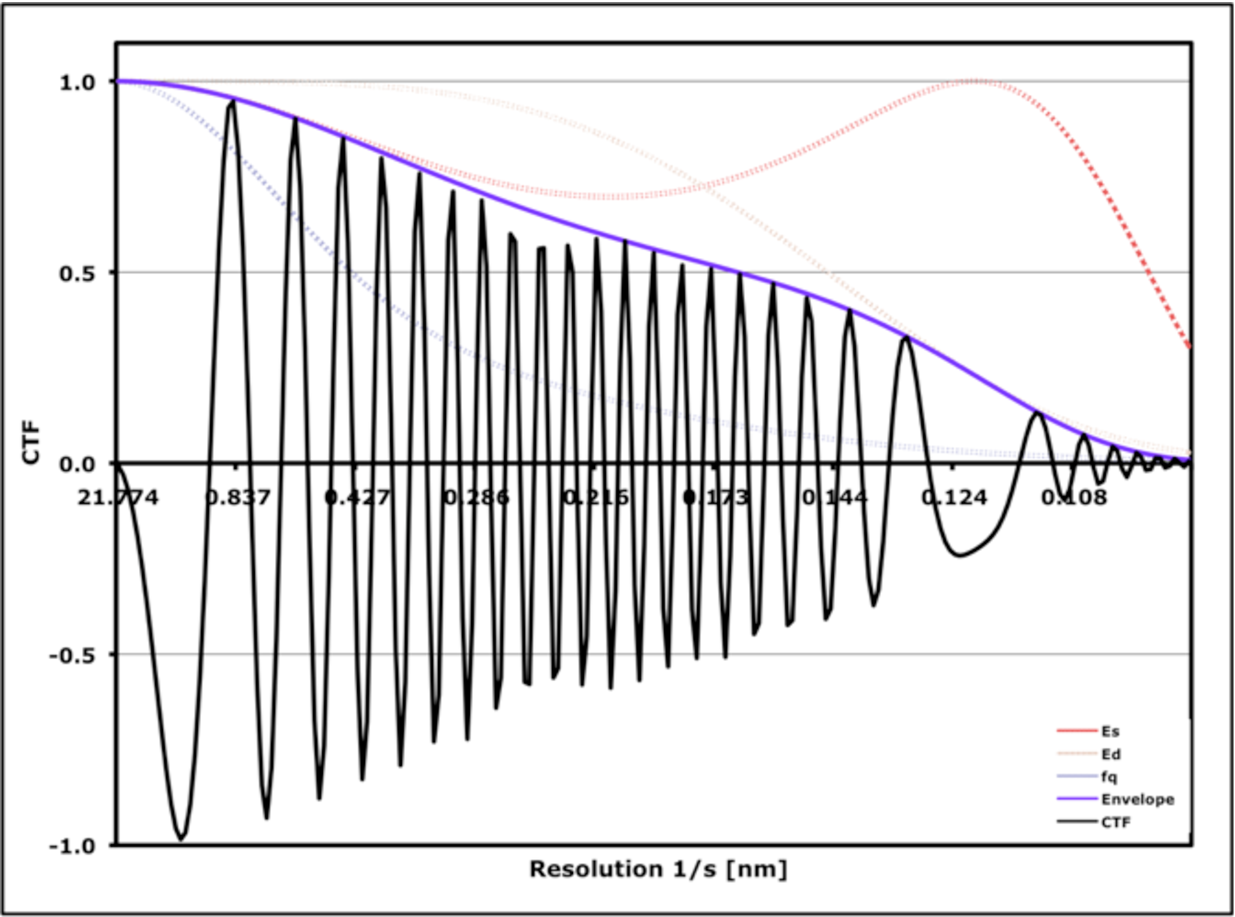
\includegraphics[width=.85\textwidth]{ctf.pdf}
		\caption{Example of a Contrast Transfer Function}
		\label{fig:ctf}
	\end{figure}
	
\newpage

\subsubsection{Space Group Determination}	
\index{Space Group Determination}
\label{sec:space_group}

CTF-corrected data can always be combined in "plane group p1", i.e. assuming no symmetry at all. However, if the specimen does exhibit a certain symmetry, data handling and refinement becomes a lot easier because symmetry imposes constraints on the molecular transform. For instance, a simple twofold axis of symmetry means that the densities within the unit cell are related by a 180\textdegree
rotation about this axis. Consequently, the density distribution will appear symmetrical in non-tilted image data (= projection density map). To encode this in reciprocal space requires all the projection terms to be symmetric about the origin, i.e. they are cosine waves that can only be shifted by 0 or 180\textdegree with respect to the phase origin.
The introduction of redundancy is a further advantage of symmetry. For instance the terms (1 0 0), (0 -1 0) and (-1 1 0) are all different if no symmetry is present. However, if the specimen displays three- or six-fold symmetry these terms have identical phases and amplitudes, i.e. they are symmetry related, describing the same structural feature. In other words while the data of a single image only contribute a single measurement for each reflection in the first case, three independent measurements of the "unique" reflection (= 1 0 0) are obtained for three- or six-fold symmetry. In addition, the actual phase values allow discriminating further between three- (p3) and six-fold (p6) symmetry. Since the latter has intrinsic twofold symmetry all phases would be expected to adopt 0 or 180\textdegree values. However, this is not true in p3 where like in p1 no phase constraints are applicable. The agreement between symmetry related reflections is independent of the CTF as long as the image has no significant astigmatism because they have the same distance from the transform origin. 
In summary, the relationships between the phases obtained from images of non-tilted crystals allow an unambiguous determination of the specimen's symmetry because each of the 17 plane groups has a unique set of constraints. 

To determine the space group of your crystal run the \textit{Get Spacegroup \& Phase Origin} \index{Get Spacegroup \& Phase Origin} script in the \textit{Custome Scripts} panel. It will calculate the internal phase residuals for all space groups and thereby choose the optimal space group and the corresponding phase origin. The space group and phase origin are then in \texttt{2dx\_image} as entries for \textit{Symmetry and Phase Origin} (see \autoref{fig:spacegroup}). To find the right space group it is better to set the \textit{Resolution limitation for phase origin search} to a lower resolution than with what you process your image. In case you know the space group of your crystal you can also use this script to just find the according phase origin for the image. Note that only projection images of non-tilted crystals show symmetry.

\begin{figure}
		\centering
		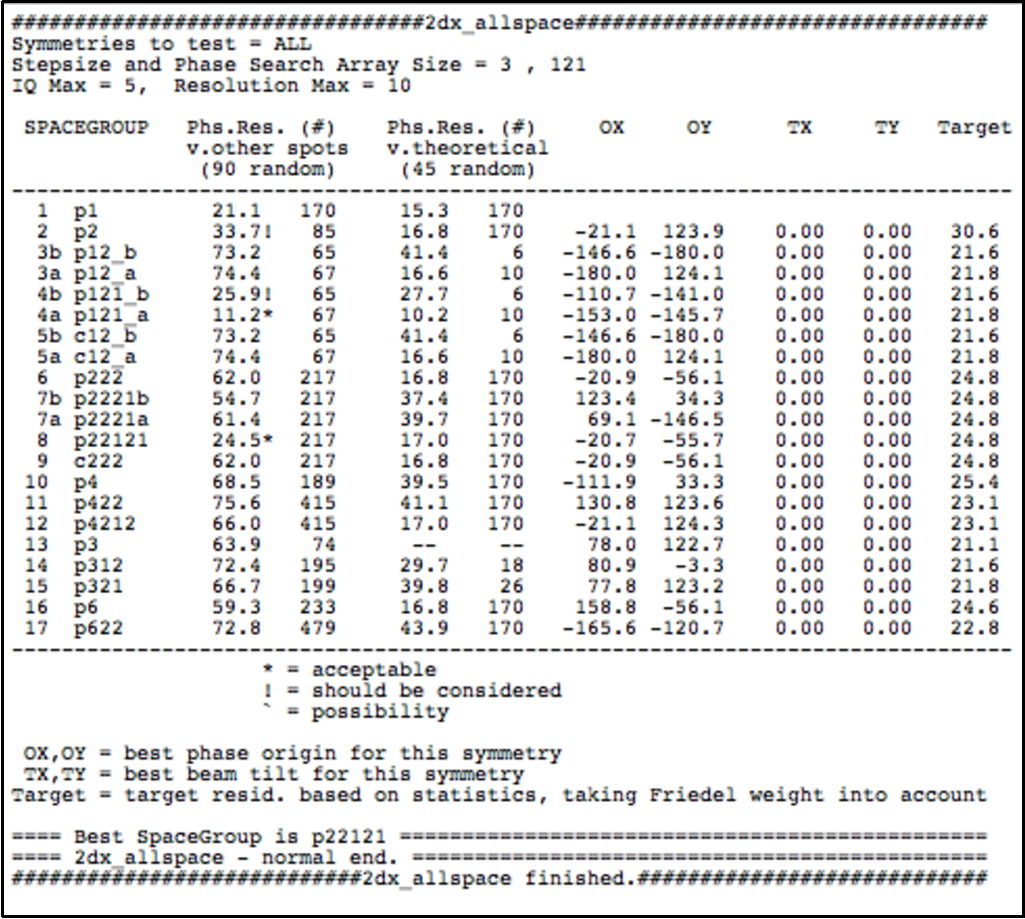
\includegraphics[width=.85\textwidth]{spacegroup.pdf}
		\caption{Example of space group determination.}
		\label{fig:spacegroup}
	\end{figure}

Optionally you can set your phase origin manually. This way you could process all your single images to a similar phase origin, making it later easier to find a common phase origin in 2D merging \autoref{sec:2d_merging}. For this purpose run the \textit{Set PhaseOrigin Manually}\index{Set PhaseOrigin Manually} script in the  \textit{Custom Script} panel. Open the  \textit{Old p<X>-symmetrized Map} in the  \textit{Image} panel. 
Position your mouse cursor on the wished phase origin and press shift "P". The needed phase origin changes will be transferred to the  \textit{Parameter} panel. To apply the changes you have to rerun the script once again.

	
\subsubsection{Map Generation}	

Final step of 2D image processing is the generation of the projection map. You can create an unsymmetrized map by running the \textit{Generate Map}\index{Generate SymMap} script in the \textit{Standard Scripts} panel. Alternatively you can generate a symmetrized map by applying the selected space group. For this run run \textit{Generate Map}\index{Generate SymMap} script in the \textit{Custom Scripts} panel. The latter will calculate a table of phase residuals during the symmetrization, from which you can judge the overall quality and resolution of your image. 

Please note that you have to set the parameter \textit{Invert contrast to the final map again} to \textit{No} in case you are processing a negative stained image, and to \textit{Yes} in case of a cryo image. 


	\begin{figure}[H]
		\centering
		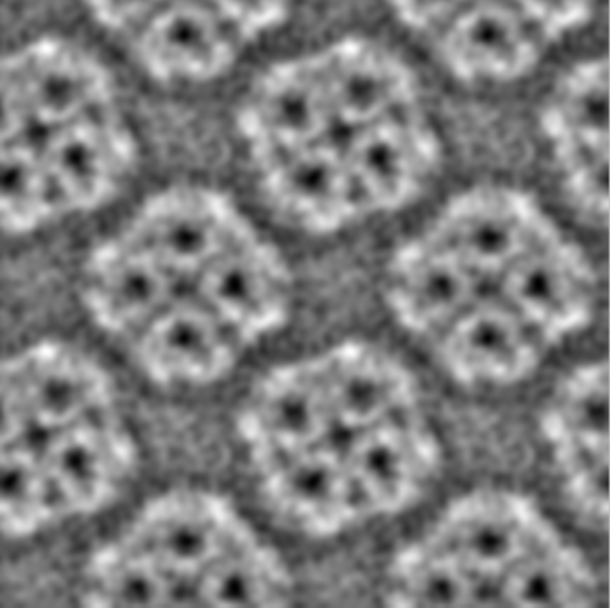
\includegraphics[width=.4\textwidth]{2d_second.pdf}
		\caption{Example of a projection map}
		\label{fig:2d_second}
	\end{figure}
	

	
		
